\documentclass{article}
\usepackage[UTF8]{ctex}
\usepackage{indentfirst}
\usepackage{graphicx}
\usepackage{amsmath}
\usepackage{xcolor}
\usepackage{tikz}
\usepackage{listings}
\usepackage{subfig}
\usepackage{geometry}
\usepackage{embrac}
\usepackage{listings}
\usepackage[framed,numbered,autolinebreaks,useliterate]{mcode}
\lstset{language=Matlab}


\usetikzlibrary{arrows,shapes,chains}
\setlength{\parindent}{2em}
\lstset{breaklines}  %让LaTeX自动将长的代码行换行排版
\lstset{extendedchars=false}   %这一条命令可以解决代码跨页时,章节标题,页眉等汉字不显示的问题
\lstset{language=Python, %用于设置语言为C++
        identifierstyle=,
        basicstyle=\ttfamily,
        stringstyle=\ttfamily,
        showstringspaces=false,
        frame=shadowbox, %边框
        captionpos=b}
\geometry{a4paper, total={170mm,257mm}, left=20mm, top=20mm,}

\begin{document}


\section{使用提供的jupyter notebook代码和环境进行Friedman检测进行初步判断,并给出是否需要进一步Nemenyi测试的判断结论,如果你的结论是需要,给出Nemenyi测试结论,并画出分布图。}

\subsection{Friedman检测初步判断}
通过修改算法比较序表和Friedman参数(共有四个数据集、五个算法),进行Friedman检测的结果为:
$$ \tau_F = 15.462  $$

在$\alpha=0.05$的置信度下,$ \tau_F = 15.462 >3.259 $,说明拒绝了所有算法性能相同假设,需要进一步进行Nemenyi测试。

\subsection{Nemenyi测试}
在$\alpha=0.05$的置信度下,设置正确的Nemeny测试参数,测到的临界值域为:

$$CD=3.05$$

观察原始算法性能表中的均值,只有算法1和算法5之间的差距超过临界值域,因此认为算法1和算法5性能有着显著差别,其余无显著差别。

\subsection{代码运行截图}

\begin{figure}[htbp]
	\centering
	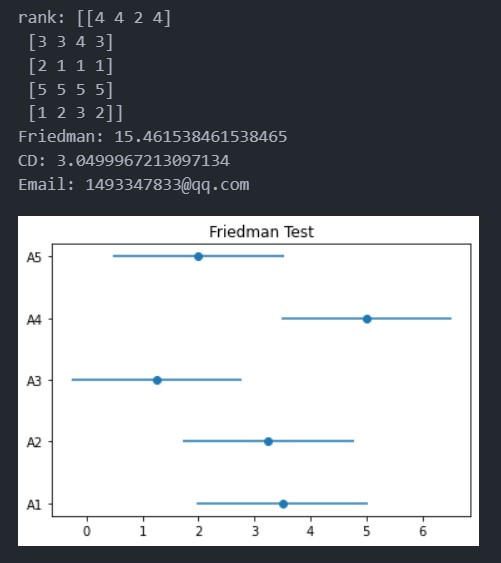
\includegraphics[scale=0.8]{1.jpg}
	\caption{代码运行结果}
	\label{figure}
\end{figure}
通过观察Nemenyi测试CD图可以明显看到算法1和算法5之间的横线段没有交叠,其余均有交叠。印证了算法1和算法5有显著差别的结论。

\section{课后习题2.2}
\subsection{10折交叉验证法}
由10折交叉验证的原理可得,要先将数据集100个样本划分为10个样本数为10的子集,并保证这10个子集数据分布尽量一致。因此训练集九份子集中正例一般占45,反例占45。根据以样本数较多为预测,样本数相同时进行随机猜测的原则,错误率为50$\%$。
\subsection{留一法}
当采用留一法时,将训练集分成100份,也就是每个样本为一份。此时若留下的样本为正例,则训练集中有49个正例50个反例,根据题目原则会将测试集预测为反例,预测错误;反之同理,也为错误。因此错误率为100$\%$。

%\section{用MATLAB分别画出对应的频率特性图,提交可运行的源码}
%\subsection{rc.m}
%\begin{lstlisting}
%	% 定义电路参数
%	RC = 2; 
%	% 定义传递函数系数
%	num = [1];
%	den= [RC 1];
%	% 定义角频率范围
%	w = logspace(-1,4,1000); 
%	% 计算频率响应
%	h = freqs(num, den, w); 
%	% 绘制频率响应曲线
%	subplot(2, 1, 1); 
%	semilogx(w, 20*log10(abs(h))); 
%	xlabel('Angular frequency (rad/s)'); 
%	ylabel('Magnitude (dB)'); 
%	title('Frequency response of RLC series circuit'); 
%	grid on; 
%	subplot(2, 1, 2); 
%	semilogx(w,angle(h)*180/pi); 
%	xlabel('Angular frequency (rad/s)'); 
%	ylabel('Phase (deg)'); 
%	grid on; 
%\end{lstlisting}
%
%\subsection{rlc.m}
%\begin{lstlisting}
%	% 定义电路参数
%	R = 100; 
%	L = 0.01; 
%	C = 0.0001; 
%	% 定义传递函数系数
%	num = [1];
%	den = [L*C R*C 1]; 
%	% 定义角频率范围
%	w = logspace(-1,4,1000); 
%	% 计算频率响应
%	h = freqs(num,den,w); 
%	% 绘制频率响应曲线
%	subplot(2,1,1); 
%	semilogx(w, 20*log10(abs(h))); 
%	xlabel('Angular frequency (rad/s)'); 
%	ylabel('Magnitude (dB)'); 
%	title('Frequency response of RLC series circuit'); 
%	grid on; 
%	subplot(2,1,2); 
%	semilogx(w,angle(h)*180/pi); 
%	xlabel('Angular frequency (rad/s)'); 
%	ylabel('Phase (deg)'); 
%	grid on; 
%\end{lstlisting}

\end{document}